\subsection{Interplay between Degeneracy and Fermion Parity}\label{sec:origin_degeneracy_odd}

\begin{figure*}
    \centering
    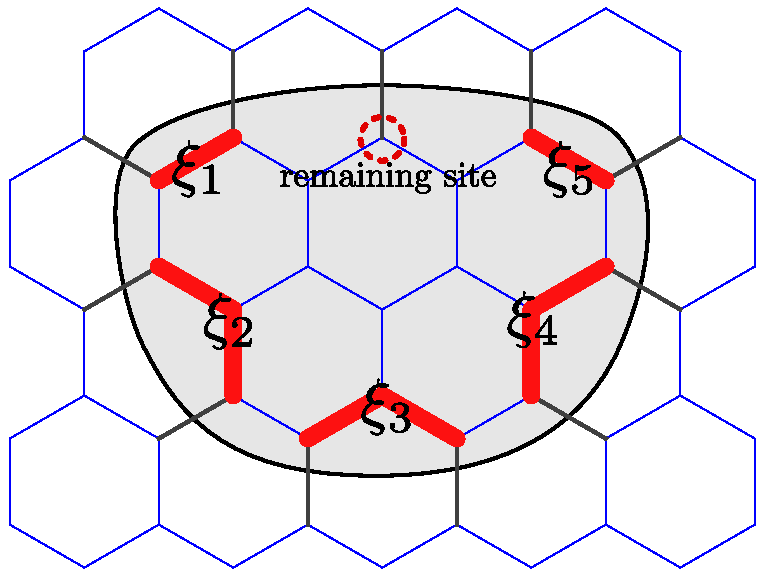
\includegraphics[width=0.25\linewidth]{figures/reshuffle-xi-def-odd.pdf}\hspace{0.5cm}
    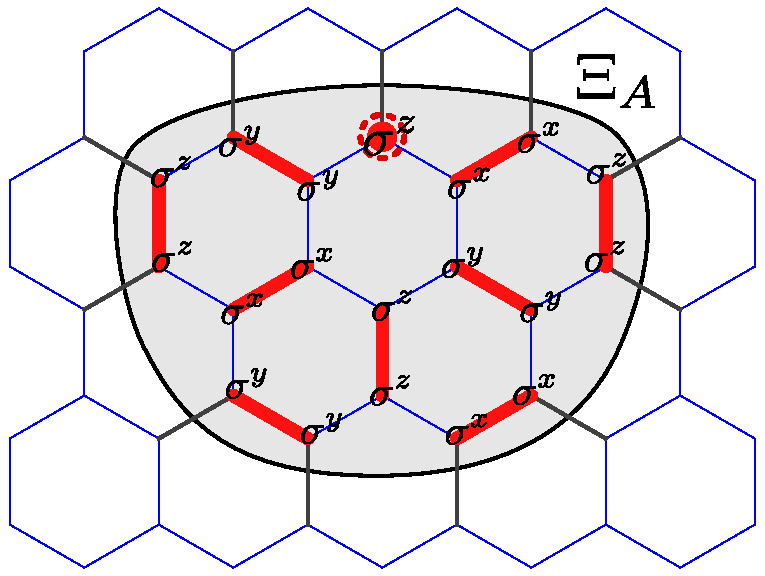
\includegraphics[width=0.25\linewidth]{figures/reshuffle-capital-Xi-def.pdf}\hspace{0.5cm}
    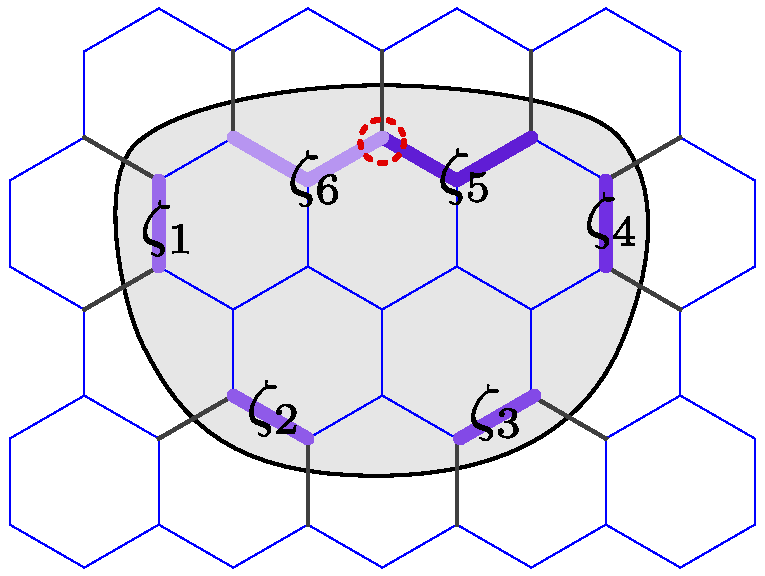
\includegraphics[width=0.25\linewidth]{figures/reshuffle-zeta-def-odd.pdf}
    \caption{For cases with odd $N^A$, there must be a single site $l$ on the boundary that remains unpaired after defining $\hat{\xi}$-operators by pairing the adjacent edges crossing the boundary, as illustrated in the left-most panel. Based on this phenomenon, we can define an operator $\hat{\Xi}_A$ in such a way that the remaining site $l$ is filled in with a Pauli matrix $\sigma^\mu_l$, where $\mu$ is the direction of the edge crossing the boundary that connects to $l$. At the same time, the rest of the part is covered by a dimer covering, as illustrated in the middle panel. On the other hand, the $\hat{\zeta}$-operators are defined in a way similar to what we have introduced, but there are two connected $\hat{\zeta}$-operators sharing one site, which is exactly $l$ after the pairing we have done to define $\hat{\xi}$-operators. In the example illustrated in the right-most panel, the two connected $\hat{\zeta}$-operators are $\hat{\zeta}_5$ and $\hat{\zeta}_6$, and we have $\hat{\zeta}_5\hat{\Xi}\hat{\zeta}_5 = \hat{\zeta}_6\hat{\Xi}_A\hat{\zeta}_6 = -\hat{\Xi}_A$.}
    \label{fig.Xi-odd}
\end{figure*}

\valert{
The notion of fermion parity obtained in Sec.~\ref{sec:EE-calculation-odd} motivates a question: how to describe fermion parity in the spin representation? And how does it give an additional degeneracy in the entanglement spectrum? In this section, we find a specific sort of operator in spin representation that corresponds to fermion parity. It further block-diagonalizes the density matrix if $N^A$ is odd, hence gives an additional degeneracy.
}

A relation implied by equation \eqref{equ.Pick_sim-con} 
\[%\label{equ.bulk-boundary-parity}
    N^A=\abs{\de A} \mod{2},
\]
indicates that once the number of lattice sites in $A$ is odd, so is the length of the boundary. This raises an issue that there will always be one single site left after sorting lattice sites along the boundary in pairs, as shown in the first panel of \autoref{fig.Xi-odd}. If $L$ is defined as the number of $\hat{\xi}$-operators, then in cases with odd $\abs{\de A}$, we onlyl have
\[
L = \frac{1}{2}\lr{\abs{\de A} - 1}
\]
In this way, the block-diagonal structure \eqref{equ.block-rho-final} and the derivation \eqref{equ.EE-from-blocks} are still valid, but the result should be modified as
\begin{align}\label{equ.EE-odd-blocks}
    S_A &= -\Tr_A\Tilde{\rho}_A\ln\Tilde{\rho}_A + \lr{L-1}\ln 2 \nonumber\\
    &= -\Tr_A\Tilde{\rho}_A\ln\Tilde{\rho}_A + \lr{\frac{1}{2}\abs{\de A}-\frac{3}{2}}\ln 2
\end{align}
where $\Tilde{\rho}_A\equiv 2^{L-1}\varrho_A$. The form of \eqref{equ.EE-odd-blocks} is the same as that of \eqref{equ.EE-odd-derive-1}, showing that the block $\Tilde{\rho}_A$ here is identical to the Majorana reduced density matrix \eqref{equ.rho-A-F-odd} with a redundant Majorana fermion included. 

In Sec.~\ref{sec:EE-calculation-odd}, the result of the Majorana entanglement spectrum shows that the degree of degeneracy is 
\[
2^{\frac{N^A+1}{2}-N^A_p} = 2^{\frac{1}{2}\lr{\abs{\de A} - 1}} = 2^L
\]
However, according to the discussion in the previous part for cases with an even number of sites, the degree of degeneracy is $2^{L-1}$ if there are $L$ well-defined $\hat{\xi}$-operators. This discrepancy implies that apart from the set of $\hat{\xi}$-operators, there exists an additional operator that further block-diagonalizes $\rho_A$ to give an additional 2-fold degeneracy to the entanglement spectrum. At the end of Sec.~\ref{sec:EE-calculation-odd}, we have elucidated that the additional 2-fold degeneracy in the entanglement spectrum of the Majorana sector originates from the total fermion parity. Therefore, we anticipate that the additional operator block-diagonalizing the density matrix, which will be denoted by $\hat{\Xi}_A$ later, should be related to the total fermion parity in the Majorana representation. A feasible choice is a dimer covering of the subregion $A$,
\begin{equation}\label{equ.Xi-def}
    \hat{\Xi}_A \equiv \sigma^\mu_l \Sigma_{\mathfrak{D}_{\mrm{DC}}^{A(l)}},
\end{equation}
where the edge configuration $\mathfrak{D}_{\mrm{DC}}^{A(l)}$ stands for a dimer covering of $A$ with a site $l$ being excluded. Since $N^A$ is an odd number, it is not possible for a dimer configuration composed of non-overlapping dimers to cover the entire subregion~\footnote{The dimer covering is not uniquely defined. One can choose an arbitrary dimer covering with a remaining site $l$ at the boundary that covers the subregion.}. The remaining site $l$ is required to be at the boundary of the subregion $A$, and the direction $\mu$ of the Pauli matrix $\sigma_l^\mu$ is that of the edge connected to $l$ that crosses the boundary. An example is illustrated in \autoref{fig.Xi-odd}, where the remaining site $l$ is in the upper portion of the subregion. 

$\hat{\Xi}_A$ can be examined to commute with $\rho_A$ in the same way as used for $\hat{\xi}$-operators. String operators are composed of multiple dimers, and every dimer commutes with the dimer covering because of the properties of Pauli matrices. Therefore, the only thing to be concerned about is $\sigma^\mu_l$ lying at the remaining site.
As we have defined, the site $l$ is at the boundary and $\mu$ points outward. It can be seen directly that, inside $A$, there are only two edges connected to $l$, and the corresponding string operator of both edges anti-commutes with $\sigma^\mu_l$. However, since the string operator also anti-commutes with the dimer that connects to the other endpoint of the edge, the two anti-commutations cancel each other. In the end, every string operator with $\mathfrak{D}\subset A$ commutes with $\hat{\Xi}_A$. Because $\rho_A$ is composed of string operators inside $A$, we conclude that $[\hat{\Xi}_A,\rho_A]=0$. 

$\hat{\Xi}_A$ is related to the total fermion parity by transforming \eqref{equ.Xi-def} into the Majorana fermion representation, and we find that it is equal to the total fermion parity operator multiplied by the gauge-field operators arranged in order of the dimer covering $\mathfrak{D}^{A(l)}_{\mrm{DC}}$
\[
\hat{\Xi}_A \propto \lr{\prod_{\anglelr{ij}\in  \mathfrak{D}^{A(l)}_{\mrm{DC}}} \hat{u}_{ij}} \lr{b^\mu_l\prod_{i\in A}c_i}
\]
up to a phase. In the above formula, the total fermion parity operator is defined as
\begin{equation}\label{equ.total-fermion-parity-odd}
    \hat{\bog{\pi}}^{(A)} \propto b^\mu_l\prod_{i\in A}c_i
\end{equation}
with a phase correction depending on the geometry of the subregion. Because the gauge has been fixed as $u_{ij}=1\;\forall\anglelr{ij}$, the expectation value of $\hat{\Xi}_A$ is completely determined by that of $\hat{\bog{\pi}}^{(A)}$. The definition of the total fermion parity here is different from what we encountered in \eqref{equ.total-fermion-parity-entire-system} and \eqref{equ.total-fermion-parity-Sigma-Z}. In fact, because $N^A$ is an odd number, $\prod_{i\in A}c_i$ itself only contains an odd number of Majorana fermions, hence not sufficient to define a fermion parity operator. This mechanism has been discussed in Sec.~\ref{sec:EE-calculation-odd}, and the alternative we adopted there is to include a redundant Majorana fermion $c_{(N^A+1)}$, and Eq.~\eqref{equ.total-fermion-parity-odd} implies that the redundant fermion is actually $b^\mu_l$ borrowed from the gauge sector. 
%The situation in which the matter sector borrows a Majorana fermion from the gauge sector is also demonstrated in the derivation procedures \eqref{equ.EE-odd-derive-1} and \eqref{equ.EE-reduce}. 
%By now, the physical meaning of the redundant fermion and its origin are clearly reflected by $\hat{\Xi}_A$. 

So far, we have $L$ distinct $\hat{\xi}$-operators and $\hat{\Xi}_A$ that commute with $\rho_A$. These operators give $2^{L+1}$ blocks labeled with a set of eigenvalues $\lrg{\xi_1,\cdots,\xi_L;\Xi_A}$. To prove that these blocks are identical, leading to extensive degeneracy, we also have to find $(L+1)$ $\hat{\zeta}$-operators that relate all the blocks in the same way as \eqref{equ.xi-zeta-relation}. Since $\hat{\zeta}$-operators do not have to commute with each other, we can still find $(L+1)$ of them, as illustrated in the last panel of \autoref{fig.Xi-odd}. The arrangement of $\hat{\zeta}$-operators is designed in a way that two of them overlap at the remaining site $l$. In this way, the $\hat{\xi}$-operators can still be flipped through \eqref{equ.xi-zeta-relation}. More importantly, both overlapping $\hat{\zeta}$-operators can flip the sign of $\Xi_A$. 
%Take \autoref{fig.Xi-odd} for example, these two overlapping operators are $\hat{\zeta}_5$ and $\hat{\zeta}_6$, by which $\hat{\Xi}_A$ can be flipped in the way that $\hat{\zeta}_5\hat{\Xi}_A\hat{\zeta}_5 = \hat{\zeta}_6\hat{\Xi}_A\hat{\zeta}_6 = -\hat{\Xi}_A$. 
%Similar to what we encountered in cases with even $N^A$, 
Since each $\hat{\zeta}$-operator simultaneously flips two values in the set $\lrg{\xi_1,\cdots,\xi_L;\Xi_A}$, they only provide $2^L$-fold degeneracy in the entanglement spectrum although we have $(L+1)$ operators to block-diagonalize $\rho_A$. This agrees with our analysis in Sec.~\ref{sec:EE-calculation-odd}, and the operator $\hat{\Xi}_A$ indeed gives a 2-fold degeneracy to the entanglement spectrum. 

\begin{figure}
    \centering
    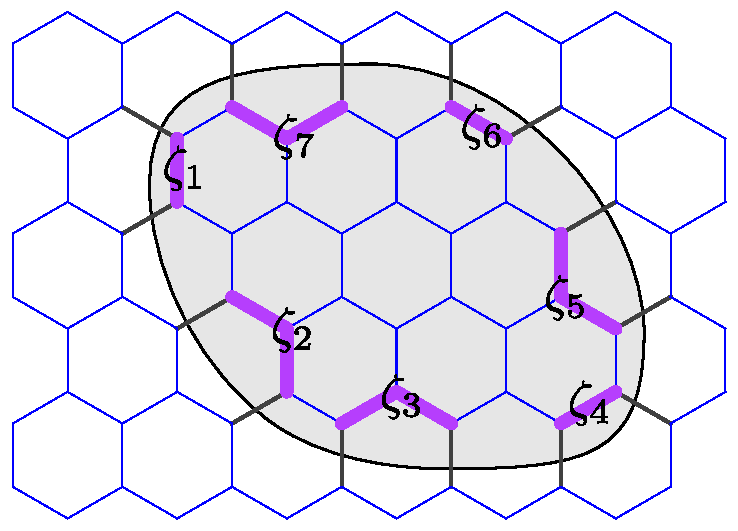
\includegraphics[width=0.4\linewidth]{figures/reshuffle-larger-zeta.pdf}\hspace{0.5cm}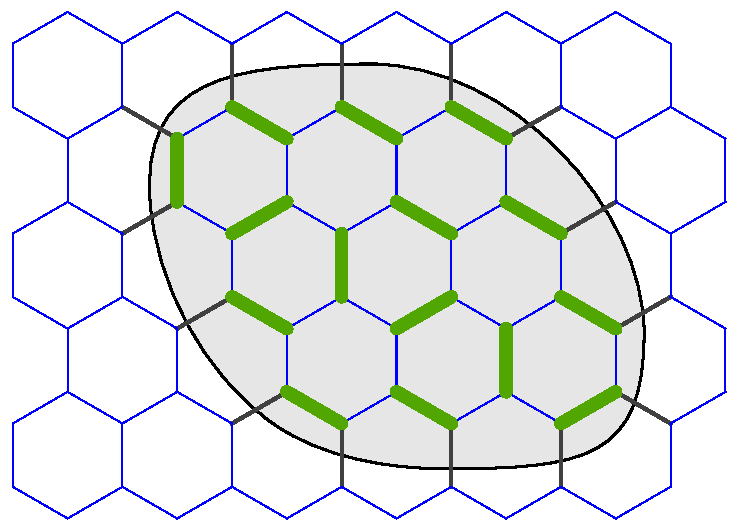
\includegraphics[width=0.4\linewidth]{figures/reshuffle-larger-dimer-covering.pdf}
    \caption{For regions with an even number of lattice sites, at least a dimer covering is well defined, like the one illustrated in the right panel. Assigning a string operator to each dimer in the configuration gives a dimer-covering string operator $\hat{\Xi}_A$ without a single unpaired site, unlike we encountered in cases with an odd number of sites. However, it can be directly checked that $\hat{\Xi}_A$ in this case commutes with every $\hat{\zeta}$-operator. Therefore, such an operator doesn't provide additional degeneracy in the entanglement spectrum.}
    \label{fig.dimer-covering}
\end{figure}
Although it seems that $\hat{\Xi}_A$ can also be defined in cases with even $N^A$ and leads to an additional 2-fold degeneracy, the operator $\hat{\Xi}_A$ defined in this way commutes with every $\hat{\zeta}$-operator, implying that no operator can relate blocks with $\Xi_A=+1$ and $\Xi_A=-1$. As illustrated in \autoref{fig.dimer-covering}, the pattern is simply a dimer covering without a remaining site.  Thus, $\hat{\Xi}_A$ cannot yield a 2-fold degeneracy in the entanglement spectrum in cases with even $N^A$. This constitutes an intrinsic difference between cases with even and odd $N^A$, which is reflected in the total fermion parity in the subregion in the Majorana representation, or equivalently in the dimer covering operator $\hat{\Xi}_A$ in the physical spin formulation.

